\documentclass[a4paper,11pt]{article}

\usepackage[utf8x]{inputenc}
\usepackage[T1]{fontenc}
\usepackage[francais]{babel}
\usepackage{amsmath,amssymb}
\usepackage{fullpage}
\usepackage{xspace}
\usepackage{verbatim}
\usepackage{graphicx}
\usepackage{listings}
\usepackage[usenames,dvipsnames]{color}
\usepackage{url}

\lstset{basicstyle=\small\tt,
  keywordstyle=\bfseries\color{Orchid},
  stringstyle=\it\color{Tan},
  commentstyle=\it\color{LimeGreen},
  showstringspaces=false}

\newtheorem{exo}{Exercice}

\newcommand{\dx}{\,dx}
\newcommand{\ito}{,\dotsc,}
\newcommand{\R}{\mathbb{R}}
\newcommand{\C}{\mathbb{C}}
\newcommand{\N}{\mathbb{N}}
\newcommand{\Poly}[1]{\mathcal{P}_{#1}}
\newcommand{\abs}[1]{\left\lvert#1\right\rvert}
\newcommand{\norm}[1]{\left\lVert#1\right\rVert}
\newcommand{\pars}[1]{\left(#1\right)}
\newcommand{\bigpars}[1]{\bigl(#1\bigr)}
\newcommand{\set}[1]{\left\{#1\right\}}

\title{TP Scilab-Latex : Compte-rendu}
\author{Michel Yoeung et Billy Ndihokubwayo (groupe 2)}
\date{22 Novembre 2017}

% ===============
\begin{document}
% ===============
\maketitle

%======================================
\section{Sensibilisation à l'arithmétique machine}
%======================================

\begin{exo} \ \\ \\
On obtient $ z=0 $ et $ w=1 $. \\
Pour z, on évalue en premier $ y+x $ : $ 1e(30)+1e(-8) $ qui vaut toujours $ 1e(30) $ (pour Scilab) car le nombre de chiffres significatifs dépasse la limite de chiffres que peut gérer Scilab. On aura par conséquent, $ 1e(30)-1e(30) $ qui vaut 0 donc $ z=0 $. \\
Pour w, on évalue en premier $ x-x $ qui vaut 0 puis $ \frac{1e(-8)}{1e(-8)} $ qui vaut 1 donc $ w=1 $.
\end{exo}

\begin{exo} \ \\
\begin{figure}[h]
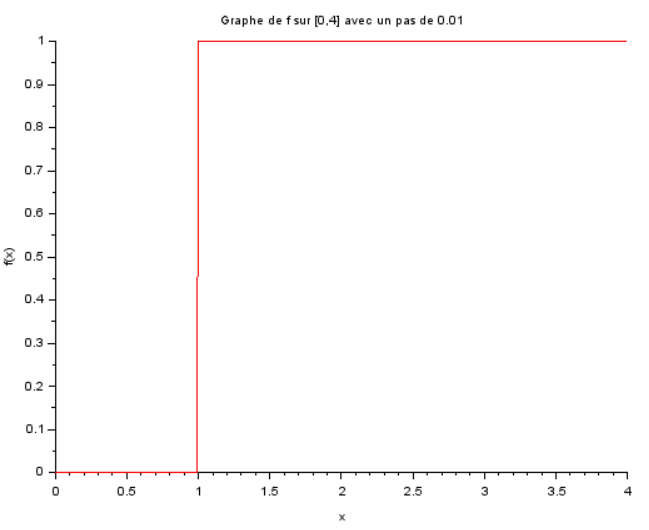
\includegraphics[scale=0.9]{../annexes/images/courbe_racine.PNG}
\end{figure} \ \\
Lorsque $ x \in [0,1[, f(x)=0 $ car lorsqu'on répète la racine, on va s'approcher de $ 1 $ mais sans jamais être égal à $ 1 $ pile (un moment donné, la valeur de la racine carrée sera bloquée à la valeur juste en dessous de $ 1 $). Donc lorsqu'on va répéter les carrés par la suite, le résultat va décroître jusqu'à atteindre $ 0 $. \ \\
Lorsque $ x=1 $, enchainer les racines carrées et les carrées ne change rien et $ f(x)=1 $ toujours. \ \\
Lorsque $ x \in ]1,4], f(x)=1 $ car lorsqu'on répète la racine carrée, le résultat va décroître jusqu'à atteindre $ 1 $. Donc, lorsqu'on va répéter les carrés par la suite, le résultat va rester à $ 1 $.
\end{exo}

\begin{exo} \ \\
\begin{enumerate}
\item On a $ I_n=\int_{0}^{1} x^ne^x \, \mathrm{d}x = e-n\int_{0}^{1} x^{n-1}e^x \, \mathrm{d}x = e-nI_{n-1} $ et $ I_0=e-1 $. \ \\
En utilisant une fonction récursive sur Scilab (probleme1.sce > suite(n)), on trouve $ I_{20}\approx\text{-}129.26 $.
\item On a $ I_n = \int_{0}^{1} x^n\sum_{k=0}^{\text{+}\infty} \left (\frac{x^k}{k!} \right) \, \mathrm{d}x = \int_{0}^{1} \sum_{k=0}^{\text{+}\infty} \left (\frac{x^{k+n}}{k!} \right) \, \mathrm{d}x = \int_{0}^{1} \lim_{N\to\\{\text{+}\infty}}\sum_{k=0}^{N} \left (\frac{x^{k+n}}{k!} \right) \, \mathrm{d}x $. \ \\
D'après le théorème de Beppo-Levi, on obtient $ I_n = \lim_{N\to\\{\text{+}\infty}}\sum_{k=0}^{N} \left(\int_{0}^{1} \frac{x^{k+n}}{k!} \, \mathrm{d}x \right) \newline = \lim_{N\to\\{\text{+}\infty}}\sum_{k=0}^{N} \left(\frac{1}{k!}[\frac{x^{k+n+1}}{k+n+1}]_0^1 \right) = \lim_{N\to\\{\text{+}\infty}}\sum_{k=0}^{N} \left(\frac{1}{k!(k+n+1)} \right) $. \ \\
En calculant cette somme jusqu'à $ N=10000 $ sur Scilab (probleme1.sce > serie\_exp(n)), on trouve $ I_{20}\approx0.1238 $.
\item Il vaut mieux donc utiliser la série exponentielle plutôt que la récurrence car en utilisant la fonction récursive, on cumule $ 20 $ fois les erreurs de précision de Scilab pour finalement obtenir un résultat incohérent de $ I_{20} $.
\end{enumerate}
\end{exo}

\begin{exo} \ \\ \\
On sait que $ \int_{a}^{b} f(x) \, \mathrm{d}x = \lim_{N\to\\{\text{+}\infty}}\sum_{k=0}^{N} \left(\frac{b-a}{N}f(a+k\frac{b-a}{N}) \right) $. \ \\
On a donc $ I_{20} = \int_{0}^{1} x^{20}e^x \, \mathrm{d}x = \lim_{n\to\\{\text{+}\infty}}\sum_{k=0}^{n} \left(\frac{1}{n}(\frac{k}{n})^{20}e^{\frac{k}{n}} \right) $. \ \\
En calculant cette somme jusqu'à $ n=100000 $ sur Scilab (probleme1.sce > rectangle(n)), on trouve $ I_{20}\approx0.1238 $ ce qui correspond au résultat trouvé en 3.2.
\end{exo}

%======================================
\section{Etude du phénomène de Gibbs}
%======================================

\begin{exo} \ \\ \\
f une fonction 1-périodique sur $ [-\frac{1}{2},\frac{1}{2}[ $. \ \\
On calcule : \ \\
$ a_0(f) = 1\int_{\text{-}\frac{1}{2}}^{\frac{1}{2}} f(x) \, \mathrm{d}x = \text{-}\int_{\text{-}\frac{1}{2}}^{0} \, \mathrm{d}x + \int_{0}^{\frac{1}{2}} \, \mathrm{d}x = 0 $. \ \\
$ a_n(f) = 2\int_{\text{-}\frac{1}{2}}^{\frac{1}{2}} f(x)cos(2\pi nx) \, \mathrm{d}x = \text{-}2\int_{\text{-}\frac{1}{2}}^{0} cos(2\pi nx) \, \mathrm{d}x + 2\int_{0}^{\frac{1}{2}} cos(2\pi nx) \, \mathrm{d}x = 0 $. \ \\
$ b_n(f) = 2\int_{\text{-}\frac{1}{2}}^{\frac{1}{2}} f(x)sin(2\pi nx) \, \mathrm{d}x = \text{-}2\int_{\text{-}\frac{1}{2}}^{0} sin(2\pi nx) \, \mathrm{d}x + 2\int_{0}^{\frac{1}{2}} sin(2\pi nx) \, \mathrm{d}x = \frac{\text{-}cos(\pi n)-cos(\pi n)+2}{\pi n} $ \ \\
\text{\enspace\enspace\enspace\space\space} $ = \frac{\text{-}2(\text{-}1)^n+2}{\pi n} $. \ \\
On obtient la série de Fourier $ f(x) = \frac{2}{\pi}\sum_{n=1}^{\text{+}\infty} \left(\frac{\text{-}(\text{-}1)^n+1}{n}sin(2\pi n x) \right) $. \ \\
$ \frac{\text{-}(\text{-}1)^n+1}{n} $ va s'annuler lorsque n est pair, donc il faut que n soit impair ($ n = 2n+1, n\in\mathbb{Z} $). \ \\
D'où $ f(x) = \frac{4}{\pi}\sum_{n=0}^{\text{+}\infty} \left(\frac{sin(2(2n+1)\pi x)}{2n+1} \right) $ qui s'annule lorsque $ x = 0 $. \ \\
Donc la formule ci-dessus est valide lorsque $ x\in[\text{-}\frac{1}{2},0[\cup]0,\frac{1}{2}[ $.
\end{exo}

\newpage
\begin{exo} \ \\ \\

\begin{figure}[h]
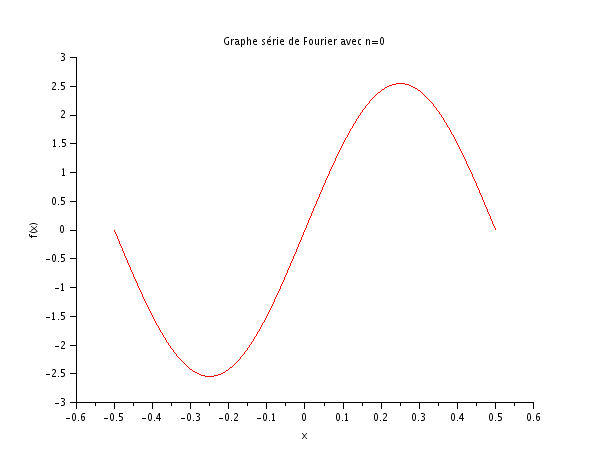
\includegraphics[scale=0.5]{../annexes/images/fourier_0.PNG}
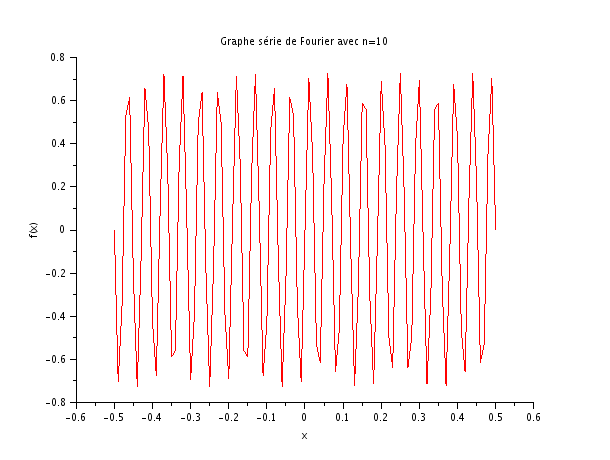
\includegraphics[scale=0.5]{../annexes/images/fourier_10.PNG}
\end{figure} \ \\



\end{exo}

% =============
\end{document}
% =============
